%%%%%%%%%%%%%%%%%%%%%%%%%%%%%%%%%%%%%%%%%%%%%%%%%%%%%%%%%%%%%%%%%%%%%%%%%%%%%%
%
% Section file included in main project file using \input{}
%
% Assumes that LaTeX2e macros and packages defined in cg_comp.sty are
%   available
%
%%%%%%%%%%%%%%%%%%%%%%%%%%%%%%%%%%%%%%%%%%%%%%%%%%%%%%%%%%%%%%%%%%%%%%%%%%%%%%

 \section{Experimental Estimate of the String Constant\label{sct:exp}}

 \begin{equation}
 \begin{split}
L_{n \ge 1}(y) &= \sqrt{\left(X_n + \Delta S\right)^2 + (b + c)^2 + y^2} \\
&\approx X_n + \Delta S + \frac{(b + c)^2 + y^2}{2\, X_n}\, .
 \end{split}
 \end{equation}

 \begin{equation}
 \begin{split}
L^\prime_{n \ge 1}(y) &= \sqrt{\left(X_0 - X_n + \Delta N\right)^2 + b^2 + y^2} \\
&\approx X_0 - X_n + \Delta N + \frac{b^2 + y^2}{2 \left(X_0 - X_n\right)}\, .
 \end{split}
 \end{equation}

 \begin{equation}
 \begin{split}
\lambda_n(y) &\approx \frac{1}{2\, X_0} \left[ \frac{(b + c)^2 + y^2}{X_n} + \frac{b^2 + y^2}{X_0 - X_n} - \frac{c^2}{X_0} \right] \\
&= \lambda_n(0) + \Delta \lambda_n(y) \, ,
 \end{split}
 \end{equation}
where $\lambda_n(0)$ is given by \eqn{lambda_n_approx}, and
 \begin{equation}
\Delta \lambda_n(y) \equiv \frac{1}{2 \left(\gamma_n - 1\right)}\, \left(\frac{\gamma_n\, y}{X_0}\right)^2\, .
 \end{equation}

Following the same approach we used to derive \eqn{quad_shift}, we can derive the change in the total shift due to both resonant length and linear mass density for a transverse displacement $y$. To second order in $y$, we find that
 \begin{equation}
\Delta \nu_n(y) \approx \frac{600}{\ln(2)}\, \frac{3 - 2 \gamma_n}{2 \left(\gamma_n - 1\right)}\, \left(\frac{\gamma_n\, y}{X_0}\right)^2\, .
 \end{equation}
We have plotted this expression for the first 12 frets and $y = 5$~mm in \fig{quad_shift_factory}. This shift is quite small compared to the experimental errors we'll obtain in the shifts due to tension, and we ignore it in what follows.

 \begin{figure}
  \centering
  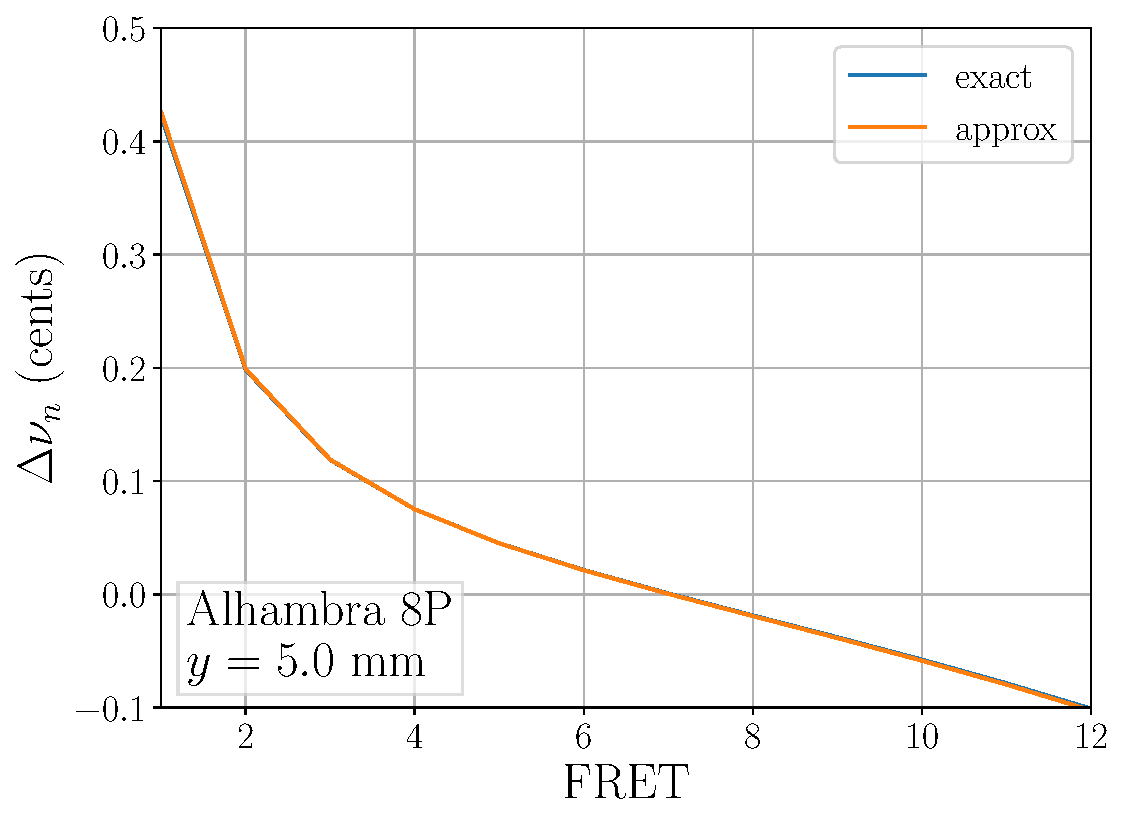
\includegraphics[width=5.0in]{figures/quad_shift_factory}
  \caption{\label{fig:quad_shift_factory} Total frequency shift (in cents) due to resonant length and linear mass density for a transverse displacement of $y = 5$~mm. This shift is identical for each string, and should be smaller than the experimental errors we'll accumulate using our transverse displacement approach.}
 \end{figure}

\begin{table}%[htbp]
  \centering
  \caption{\label{tbl:ej45_mod} Effective Young's Modulus for the D'Addario Pro-Arte Nylon Classical Guitar Strings -- Normal Tension (EJ45). The corresponding scale length is 650 mm. \red{Note that these estimates are reasonable but not quite as credible as we'd like, particularly given the effort required to obtain them. We expect the moduli of the first three strings to be the same, but they differ by as much as 40\%.}}
    \begin{tabular}{lc}
    \hline \hline
    String  & \multicolumn{1}{l}{Modulus (GPa)} \\
    \hline
    J4501 & 13.8 \\
    J4502 & 10.9 \\
    J4503 & 9.86 \\
    J4504 & 11,3 \\
    J4505 & 8.09 \\
    J4506 & 5.71 \\
    \hline
    \end{tabular}%
  \label{tab:addlabel}%
\end{table}%

% \begin{figure}
%  \centering
%  \begin{subfigure}[b]{0.8\textwidth}
%   \centering
%   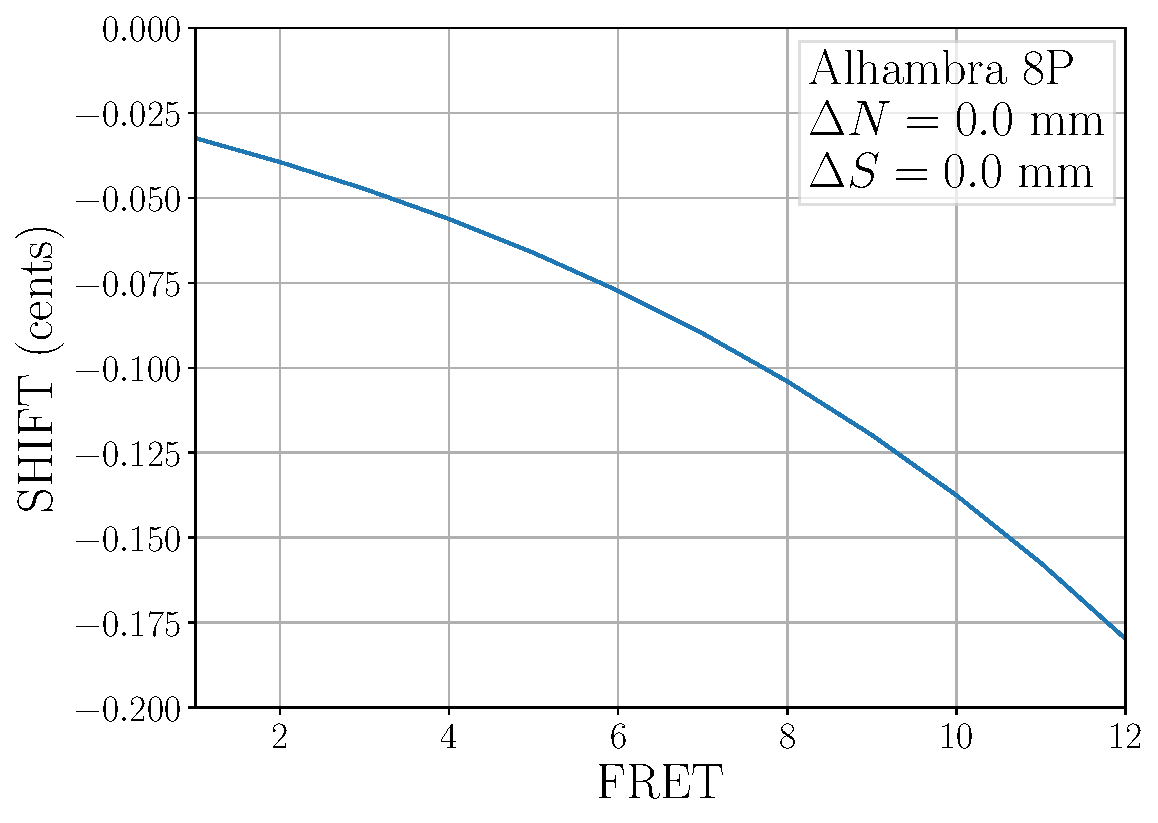
\includegraphics[width=5.0in]{figures/norm_error_uncompensated}
%   \caption{Frequency shift for an uncompensated guitar}
%   \label{fig:norm_error_uncompensated}
%  \end{subfigure}
%  \par\vspace{0.25in}
%  \begin{subfigure}[b]{0.8\textwidth}
%   \centering
%   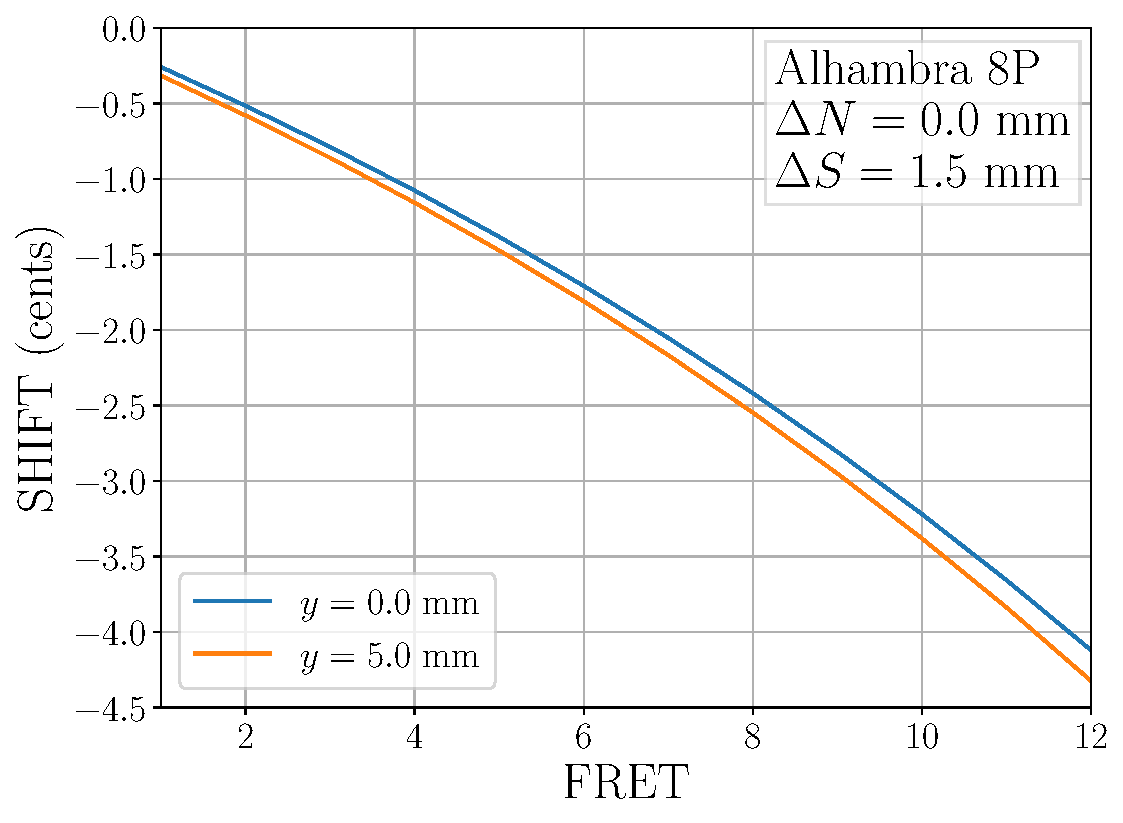
\includegraphics[width=5.0in]{figures/norm_error_factory}
%   \caption{Frequency shift for a factory guitar}
%   \label{fig:norm_error_factory}
%  \end{subfigure}
%  \caption{\label{fig:norm_error} Frequency shift (in cents) due to the fretted length $L_n$ for an uncompensated (a) and factory (b) Alhambra 8P guitar, for both zero and nonzero lateral displacement $y$.}
% \end{figure}
%
 \begin{figure}
  \centering
  \begin{subfigure}[b]{0.8\textwidth}
   \centering
   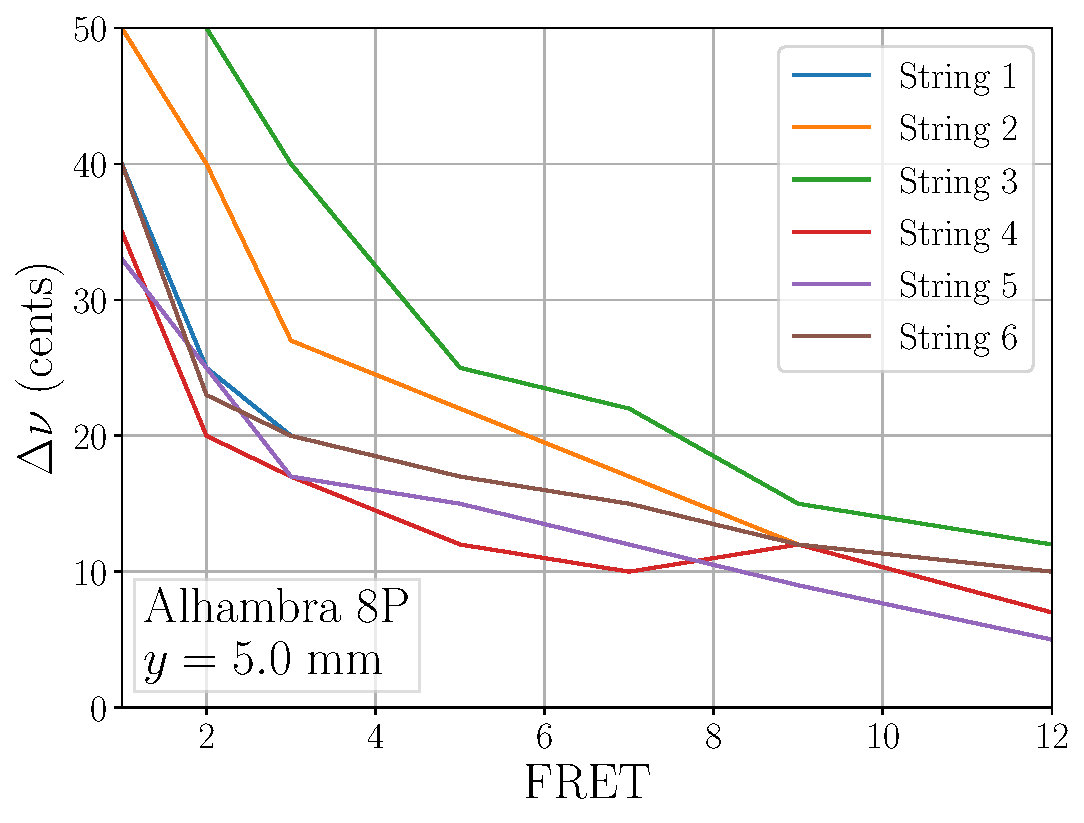
\includegraphics[width=5.0in]{figures/shift_data}
   \caption{Experimental data}
   \label{fig:shift_data}
  \end{subfigure}
  \par\vspace{0.25in}
  \begin{subfigure}[b]{0.8\textwidth}
   \centering
   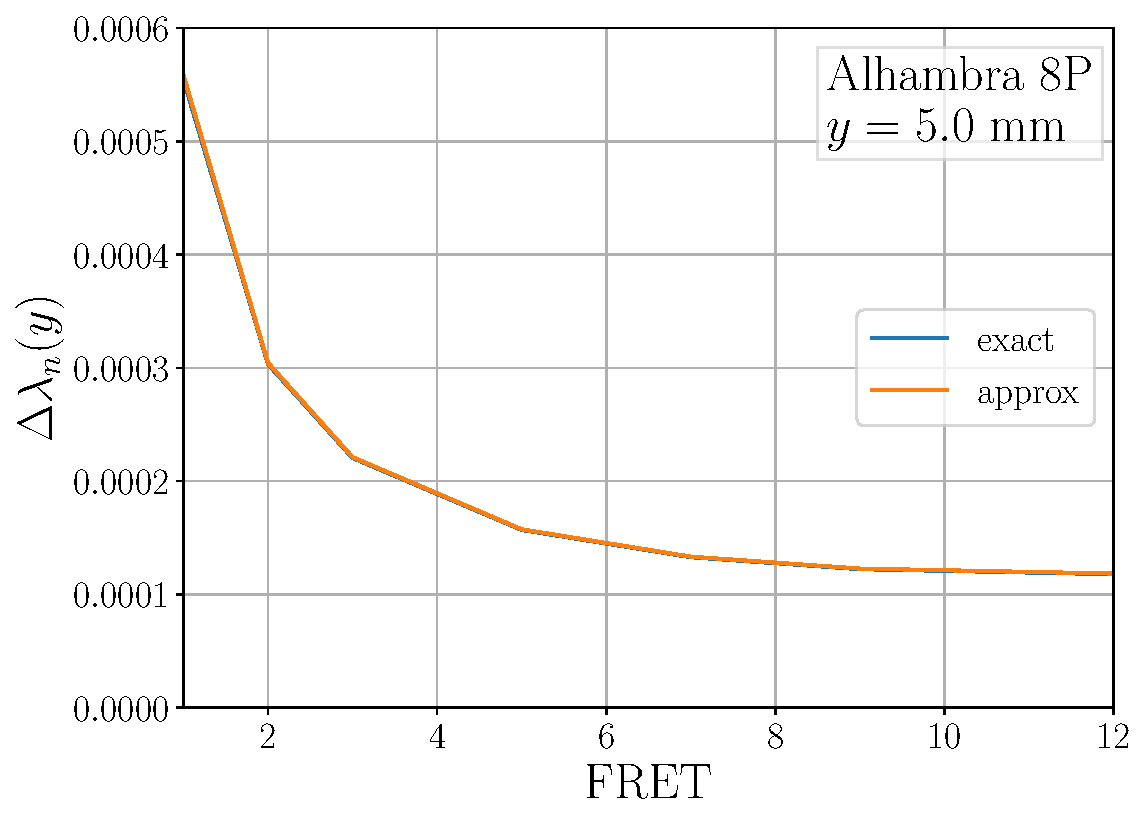
\includegraphics[width=5.0in]{figures/delta_lambda}
   \caption{Calculated change in total string length $\mathcal{L}$}
   \label{fig:delta_l}
  \end{subfigure}
  \caption{\label{fig:exp_data} Frequency shift (in cents) (a) and change in total string length $\mathcal{L}$ (b) due to lateral displacement $y$.}
 \end{figure}
